\chapter{\textsc{Identification et analyse du procédé}}
\addcontentsline{toc}{chapter}{\textsc{Identification et analyse du procédé}}


\section{\textsc{Identification des coefficients $K_m$ et $T_m$}}

\par Grâce à un oscilloscope, on obtient des signaux comme montré sur la figure ci-desous :

\begin{figure}[h!]
\centering
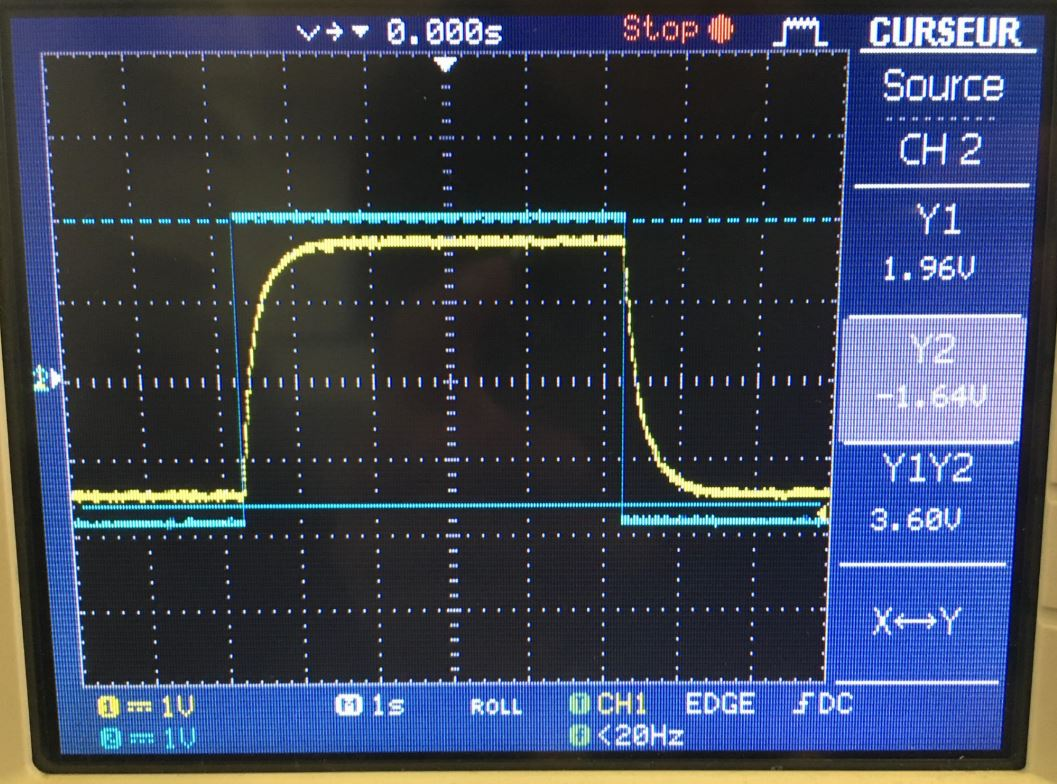
\includegraphics[scale = 0.5]{trace_temp_syst.JPG}\\[1 cm] 
\caption{Tracé temporelle du système}
\end{figure}

\par Tout d'abord nous avons mesurés le temps de monté du signal à $t_m=130ms=0.13sec$ à l'aide des curseurs (90 pour cent de la valeur finale). Afin de trouver $T_m$ nous avons utilisé une relation définit par $T_m=3*\tau$. \\

\par Or $\tau=\frac{0.13*63}{100}=0.0819sec$. Donc \fbox{$T_m=3*\tau=0.26$}\\

\par Ensuite nous avons mesuré le gain aporté sur le signal, $gain=\frac{Y_2}{Y_1}=0.837$. Or d'après le schéma de la figure 2, on a $gain=K_gK_m$ et $K_g=0.105$. Donc \fbox{$K_m=\frac{gain}{K_g}=\frac{0.837}{0.105}=8$} \\

\par Nous avons donc trouvé expérimentalement le gain en vitesse $K_m = 8$ et la constante de temps mécanique $T_m=0.26$.\\


\section{\textsc{Représentation et analyse de l'ensemble pour le système $S_{v_m->v_s}$}}

\paragraph{} On considère le système en boucle ouverte $S_{v_m->v_s}$, qui admet comme entrée le signal $v_m(t)$ et comme sortie le signal mesurée $v_s(t)$. En fonction de nos variables et de nos coefficients décrit précédement, nous avons définit la représentation d'état de ce système, en choisissant un vecteur d'état défini par :\\
$$x(t)=[x_1(t)~~x_2(t)]^T=[v_s(t)~~v_g(t)]^T$$

\paragraph{} D'après le schéma on a : $v_s(t)=K_s\theta_s(t)$ et $v_g(t)=K_g\dot{\theta_m}(t)$\\

\par Donc : $x_1(t)=K_s\theta_s(t)$ et $x_2(t)=K_g\dot{\theta_m}(t)$\\

\par Grâce a la relation sortie sur entrée on obtient : \Large$\frac{v_s(p)}{v_m(p)}=\frac{K_sK_m}{9p(1+T_mp)}$\\

\par \normalsize D'où : \Large$x_1(p)=\frac{K_sK_m}{9p(1+T_mp)}v_m$\\

\par \normalsize Or : \Large$\dot{\theta_m}(p)=\frac{K_m}{1+T_mp}v_m=\frac{v_g}{K_g}$\\

\par \normalsize On a donc : \Large$x_1=\frac{K_sv_g}{9pK_g}$\\

\par \normalsize D'où : \Large\fbox{$\dot{x_1}=\frac{K_s}{9K_g}v_g$}\\

\par \normalsize A partir de $v_g$ on trouve $\dot{x_2}$ : \Large$v_g=\frac{K_gK_mv_m}{1+T_mp}$\\

\par \normalsize On transforme $v_g$, ce qui donne : \Large$v_g=\frac{K_mK_g}{T_m}\frac{T_m}{T_mp+1}v_m$=$\frac{K_mK_g}{T_m}\frac{1}{p+\frac{1}{T_m}}v_m$\\

\par \normalsize D'où : \Large$v_g(p+\frac{1}{T_m})=\frac{K_mK_g}{T_m}v_m$\\

\par \normalsize On obtient donc : \Large$v_gp=\dot{v_g}$=\fbox{$\dot{x_2}=\frac{K_mK_g}{T_m}v_m-\frac{1}{T_m}v_g$}\\

\par \normalsize La représentation d'état du système ce présente comme ceci :\large
$$\dot{x}=\begin{bmatrix}\dot{x_1}\\\dot{x_2}\end{bmatrix}=\begin{bmatrix}0 && \frac{K_s}{9K_g} \\ 0 && -\frac{1}{T_m}\end{bmatrix}\begin{bmatrix}x_1\\x_2\end{bmatrix}+\begin{bmatrix}0\\\frac{K_mK_g}{T_m}\end{bmatrix}V_m$$
$$y=\begin{bmatrix}1&&0\end{bmatrix}x+0$$\\

\par \normalsize Par identification on obtient nos matrices:
$$A=\large\begin{bmatrix}0&&\frac{K_s}{9K_g}\\0&&-\frac{1}{T_m}\end{bmatrix} ; \normalsize B=\large\begin{bmatrix}0&&\frac{K_mK_g}{T_m}\end{bmatrix} ; \normalsize C=\large\begin{bmatrix}1&&0\end{bmatrix} ; \normalsize D=\large0$$\\

\par On obtient numériquement, si $T_m=0.3$ et $K_m=7$ :
$$A=\begin{bmatrix}0&&10.6\\0&&-3.33\end{bmatrix} ; \normalsize B=\begin{bmatrix}0&&2.45\end{bmatrix} ; \normalsize C=\begin{bmatrix}1&&0\end{bmatrix} ; \normalsize D=0$$
~~\\

\par Nous supposons que $v_m$=0, cela veut dire qu'il n'y aurait auncune puissance en entrée de notre système. Donc le système ne fonctionnerais pas et sera immédiatement aux points d'équilibre. C'est à dire $v_{se}(t)=0$ et $v_{ge}(t)=0$.\\

\par Supposons maintenant que $v_m=v_{m0}=constante$. Le système sera donc constamment en mouvement, donc en fonctionnement. Et n'atteindra jamais une position aux points d'équilibre.\\

\par Nous avons deux façon de déterminer si le système $S_{v_m->v_s}$ est stable ou instable, cela se fait évidemment autours des points de fonctionnement. Pour la première méthode, nous avons vu en cours que la fonction de transfert s'écrit d cette manière : \large $$PI=C(\lambda I-A)^{-1}B+D$$ \normalsize \\

\par Après transformation avec nos variables des matrices, on obtient ceci : 
\large$FT=\frac{1}{p^2+\frac{1}{T_m}p}\frac{K_sK_m}{9T_m}$ \normalsize \\

\par Par la suite nous étudions les pôles de cette fonction de transfert (le dénominateur) :
\large$p^2+p\frac{1}{T_m}=0~~<=>~~p(p+\frac{1}{T_m})=0$ \normalsize \\

\par Nous avons ici deux solutions, $p=0$ ou $p=-\frac{1}{T_m}$. On conclu dontème est instable, car on a un pôle positif (Instable si un pôle $\ge0$).\\

\par Pour la deuxième méthode, on cherche tout d'abord le "det$(\lambda I-A)$" et on calcule les $\lambda_1$ et $
\lambda_2$. Si la partie réel des $\lambda_1$ et $\lambda_2$ est négatif, alors le système est instable :
$$det(\large\begin{bmatrix}\lambda && 0 \\ 0 && \lambda \end{bmatrix} - \begin{bmatrix}0 && \frac{K_s}{9K_g} \\ 0 && -\frac{1}{T_m}\end{bmatrix}\normalsize)=0$$ \\

\par Ce qui donne : $$det\large\begin{bmatrix}\lambda && 0-\frac{K_s}{9K_g} \\ 0 && \lambda-\frac{K_s}{9K_g} \end{bmatrix}\normalsize=0$$ \\

\par Puis :
$$\lambda(\lambda-\frac{K_s}{9K_g})=0$$ \\

\par On a donc :
$$\lambda_1=0~~;~~\lambda_2=-\frac{1}{T_m}$$ \\

\par On peut donc conclure également que le système est instable.\\

\par On remarque que le système $S_{v_m->v_s}$ présente deux modes. Le mode stationnaire ($\lambda_1=0$) et le mode convergent ($\lambda_2=-\frac{1}{T_m}$).\\

\section{\textsc{Commandabilité et observabilité}}

\par Intéressons nous à la commandabilité ainsi qu'à l'observabilité du sytème $S_{v_m->v_s}$. Comme d'écrit dans l'énoncé, on a un vecteur d'état avec deux variables d'état : $$x(t)=\begin{bmatrix}x_1(t)&&x_2(t)\end{bmatrix}^T$$\\

\par On peut donc écrire : $Com=\begin{bmatrix}A&&AB\end{bmatrix}$ et $Obs=\begin{bmatrix}C\\CA\end{bmatrix}$ \\

\par D'où: $$Com = \begin{bmatrix}0&&25.7\\2.47&&0\end{bmatrix}$$\\
$$Obs = \begin{bmatrix}1&&0\\0&&10.5\end{bmatrix}$$\\

\par Aucune combinaison n'est possible afin de trouver une égalité entre colonnes ou lignes des deux matrices Observable et Commandable, ils sont tous les deux de rang 2 (= nombres de variables d'état). On peut donc en conclure que le système est commandable et observable également \label{section 1.2} \hyperref[Annexe A]{voir Annexe A.}\\

%\par Etant donné que notre système a un couple (A,B) commandable, donc il admet une représentation compagne de commande. Idem pour le couple (A,C) observable, notre système admet donc une représentation compagne d'observation.\\

%\section{\textsc{Représentation et analyse de l'ensemble pour le système $S_{v_m->v_g}$}}
%\par On considère ici le système en boucle ouverte $S_{v_m->v_g}$, qui admet comme entrée le signal $v_m(t)$ et comme sortie le signal mesurée $v_g(t)$. On avait 
%$$v_s=y=\begin{bmatrix}1&&0\end{bmatrix}\begin{bmatrix}v_s\\v_g\end{bmatrix}+0~U_m$$
%\par Avec cette sortie on a $v_g=0$. Or ici on veut en fonction de $v_g$ (car on étudie sur le système $S_{v_m->v_g}$). Donc seul la matrice C change, et l'espace d'état dynamique d'entré $\dot{x}(t)$ ne change pas : $$C=\begin{bmatrix}0&&1\end{bmatrix}$$\\
%~~\\
%\par Afin d'étudier la stabilité du système nous avons uniquement besoin de la matrice A, et calculer le déterminant de $(\lambda I-A)$. Or la matrice A n'a pas changé, et ce déterminant a déjà été calculé précédement. Les propriétés de stabilité du système $S_{v_m->v_g}$ reste identique à celles du système $S_{v_m->v_s}$. Le nouveau système considéré est donc stable.\\
%~~\\
%\par De même, le nouveau système considéré est commandable. Car le couple de commande (A,B) est toujours de rang 2. Cependant on ne peut pas en dire pareil pour son observabilité :
%$$Obs=\begin{bmatrix}C\\CA\end{bmatrix}=\begin{bmatrix}0&&1\\0&&-\frac{10}{3}\end{bmatrix}$$
%\par On remarque ici que cette matrice est de rang 1. Elle n'est donc pas observable, car il existe une combinaison permettant de passer d'une colonne à l'autre $->$ fois 0 (idem pour les lignes).
%\par Ce résultat était prévisible car la matrice C a changé et qu'on a une colonne nulle.
%
%\pagebreak
